%%% Version 3.4 Generated 2022/06/14 %%%
%%% You will need to have the following packages installed: datetime, fmtcount, etoolbox, fcprefix, which are normally inlcuded in WinEdt. %%%
%%% In http://www.ctan.org/ you can find the packages and how to install them, if necessary. %%%
%%%  NB logo1.jpg is required in the path in order to correctly compile front page header %%%

%\documentclass[utf8]{FrontiersinHarvard}

%
% PLEASE NOTE WE USE ACMART TEMPORARILY SO WE CAN SEE THE TOC
%
%\documentclass[utf8]{acmart} % for articles in journals

\documentclass[utf8]{FrontiersinVancouver} % for articles in journals

\usepackage{etoolbox} 
\newbool{SUBMISSION}
%\boolfalse{SUBMISSION}
\booltrue{SUBMISSION} 

\DeclareGraphicsExtensions{.pdf,.png,.jpg}

% \DeclareGraphicsExtensions{.jpg,.pdf,.png}


%\documentclass[utf8]{frontiersinFPHY_FAMS} % Vancouver Reference
%Style (Numbered) for articles in the journals "Frontiers in Physics"
%and "Frontiers in Applied Mathematics and Statistics"

\setcitestyle{square} % for articles in the journals "Frontiers in Physics" and "Frontiers in Applied Mathematics and Statistics" 


\usepackage{tcolorbox}
\usepackage{url}
\usepackage{lineno}
\usepackage[hidelinks]{hyperref}
\usepackage{microtype}
\usepackage{subcaption}
\usepackage[onehalfspacing]{setspace}
\usepackage{comment}
\usepackage[color=pink]{todonotes}
\usepackage{fancyvrb}
% \usepackage[table]{xcolor}
\usepackage{xcolor}
\usepackage[T1]{fontenc}
\usepackage{listings}
\usepackage{makecell}
\usepackage{pifont}

\usepackage{tikz}
\usetikzlibrary{mindmap,trees,arrows.meta,shadows}


\usepackage{forest}
\usepackage{hyperref}
\usepackage{adjustbox}

\usetikzlibrary{arrows.meta,shadows}

\newcommand{\ngreen}{bottom color=green!20}
\newcommand{\ngrey}{bottom color=gray!20}
\newcommand{\nred}{bottom color=red!20}
\newcommand{\nwhite}{bottom color=white!20}
\newcommand{\TODO}[1]{\todo[inline]{#1}}
\newcommand{\GVL}[1]{{\begin{blue} #1}}
\newcommand{\REPLACE}[2]{{\color{red}\it #1} \begin{quote}{\color{blue}#2}\end{quote}}
%\newcommand{\REPLACE}[2]{\begin{quote}\textcolor{red}{#1}\end{quote}\\{\textcolor{blue}{#2}}

%\usepackage[linguistics]{forest}
\usepackage{smartdiagram}

%\setcounter{secnumdepth}{6}
%\setcounter{tocdepth}{6}

\forestset{
  skan tree/.style={
    for tree={
      drop shadow,
      text width=3cm,
      grow'=0,
      rounded corners,
      draw,
      top color=white,
      bottom color=blue!20,
      edge={Latex-},
      child anchor=parent,
      %parent anchor=children,
      anchor=parent,
      tier/.wrap pgfmath arg={tier ##1}{level()},
      s sep+=2.5pt,
      l sep+=2.5pt,
      edge path'={
        (.child anchor) -- ++(-10pt,0) -- (!u.parent anchor)
      },
      node options={ align=center },
    },
    before typesetting nodes={
      for tree={
        content/.wrap value={\strut ##1},
      },
    },
  },
}
%\usepackage[linguistics]{forest}
\usepackage{smartdiagram}


\usepackage{forest}



\lstset{
  % basicstyle=\scriptsize\ttfamily,
  basicstyle=\fontsize{10}{10}\ttfamily,
  breaklines=true,
  keywordstyle=\color{BrickRed},
  moredelim=[s][\color{BrickRed}]{\{}{\}},
  % moredelim=[s][\bfseries]{workflow:}{\n},
  % moredelim=[s][\bfseries]{nodes:}{\n},
  % literate={\{}{{\textbf{\{}}}1
  % literate={workflow:}{{{\bfseries workflow:}}}9,
  % literate={nodes:}{{{\bfseries nodes:}}}6,
  escapeinside={(*}{*)}
}

% these do not use shell escape!
% therefore they are arxiv safe

\lstdefinestyle{python}{
  language=Python,
  basicstyle=\scriptsize\ttfamily,
  keywordstyle=\color{blue},
  commentstyle=\color{green!50!black},
  stringstyle=\color{Bittersweet},
  showstringspaces=false,
  breaklines=true
}

\lstdefinestyle{sh}{
  language=sh,
  basicstyle=\scriptsize\ttfamily,
  keywordstyle=\color{blue},
  commentstyle=\color{green!50!black},
  stringstyle=\color{Bittersweet},
  showstringspaces=false,
  breaklines=true,
  keywords={singularity,echo,cms,export,cd,mkdir,nvidia-smi,python,seff}
}


\newcommand{\YES}{\ding{51}}
\newcommand{\NO}{$\times$}

% \makeatletter\newcommand{\tableofcontents}{\@starttoc{toc}}\makeaother


\linenumbers


\def\keyFont{\fontsize{8}{11}\helveticabold }

\def\firstAuthorLast{von Laszewski {et~al.}} 
\def\Authors{Gregor von Laszewski\,$^{1,*}$,
Wesley Brewer,$^{3}$
Andrew Shao,$^{4}$
Christine R. Kirkpatrick,$^{4}$
% J.P. Fleischer,$^{1}$
% Harshad Pitkar,,$^{5}$
Geoffrey. C. Fox$^{1}$
}

% Affiliations should be keyed to the author's name with superscript
% numbers and be listed as follows: Laboratory, Institute, Department,
% Organization, City, State abbreviation (USA, Canada, Australia), and
% Country (without detailed address information such as city zip codes
% or street names).

% If one of the authors has a change of address, list the new address
% below the correspondence details using a superscript symbol and use
% the same symbol to indicate the author in the author list.

\def\Address{$^{1}$
Biocomplexity Institute,
University of Virginia,
% Town Center Four,
% 994 Research Park Boulevard,
 Charlottesville, VA, 22911, USA

$^{2}$
Oak Ridge National Laboratory,
P.O. Box 2008,
Oak Ridge, TN 37831, USA

$^{3}$
Hewlett Packard Enterprise Canada,
Victoria, British Columbia, Canada

$^{4}$
San Diego Supercomputer Center, UC San Diego, La Jolla, CA, 92093, USA

% $^{5}$
% Cummins
% Columbus, IN 47201
% City, State, USA
}


% The Corresponding Author should be marked with an asterisk Provide
% the exact contact address (this time including street name and city
% zip code) and email of the corresponding author

\def\corrAuthor{Gregor von Laszewski, Biocomplexity Institute,
University of Virginia,
Town Center Four,
994 Research Park Boulevard,
 Charlottesville, VA, 22911, USA
}

\def\corrEmail{laszewski@gmail.com}

\newcommand{\TITLE}{Experiment Execution in Support of Community Benchmarks Workflows for HPC}


\begin{document}

% outcomment toc when submitting

\onecolumn

% \begin{comment}
%
% FOR FINAL VERSION OUTCOMMENT
%
%\clearpage

%\listoftodos
\setcounter{tocdepth}{4}
\makeatletter\newcommand{\tableofcontents}{\@starttoc{toc}}\makeaother


{\bf \TITLE}

{\Authors}

{\Address}

\bigskip

\tableofcontents

%
% OUTCOMMENT LINES ABOVE
%
%\end{comment}

\title{\TITLE}

\firstpage{1}

\author[\firstAuthorLast ]{\Authors} %This field will be automatically populated
\address{} %This field will be automatically populated
\correspondance{} %This field will be automatically populated

\extraAuth{}

% If there are more than 1 corresponding author, comment this line and
%uncomment the next one.  \extraAuth{corresponding Author2
%\\ Laboratory X2, Institute X2, Department X2, Organization X2,
%Street X2, City X2 , State XX2 (only USA, Canada and Australia), Zip
%Code2, X2 Country X2, email2@uni2.edu}


\maketitle

% For Original Research Articles \citep{conference}, Clinical Trial
% Articles \citep{article}, and Technology Reports \citep{patent}, the
% introduction should be succinct, with no subheadings \citep{book}. For
% Case Reports the Introduction should include symptoms at presentation
% \citep{chapter}, physical exams and lab results \citep{dataset}.


% \newpage

\begin{abstract}

\section{}

leadership class computing add ... term and section
difference between doe and NSF .... ??? I do not even know. 
fairly large machines no matter if doe or not
order of 1000+ nodes we need to come up with some definition

university HPC vs Leadership class
tier-0 hpc agglomerated in top 500 which in top 500?

put link her of definitan.

define scale
also distingushed by examples.


hyperscale = datacenter mace 2.2 into 2.4 


\citep{cloudmesh-ee}

issue how to get urls into refernces.

development challang section



Over many decades High Performance Computing systems have been made available to the research community through research activities as well as commercially available solutions. The use of such systems has traditionally been restrictive due to the high costs of computing resources as well as the complex software to offer them efficiently to the community. Over time we saw also the utilization of federated resources such as Grids, Clouds, and todays hyperscale data centers. Still despite the many software systems and frameworks in support of these resources the utilization of them has been a challange, especially in the academic community educating the next generation of scientists. We also found that the use of benchmarks on various machines even if they are not federated play a significant hurdle in advertising a compute resource capability to the community. While popular frameworks such as Gatways and on the other spectrum Jupyter notebooks promise the simplification of the use, It is still important that scientific benchmarks are available that outline how such machines can be best utilized. This is best done in the form of workflow templates for the scientific application that can then be adapted accordingly to other scientific applications.

Within this paper, we focus first on identifying some very common usage patterns that outline which workflow templates that we have found most useful.. Naturally there are many other patterns available that may be addressed by other frameorks. However, we focus here on templates that have been common to us based on decades of use of HPC system dating back to the early parallel computers.
We especially have learned from our experience with the MLCommons Science working group that these issues are of significance and addressing them through simple tools improves the readiness of the community. Hence they can be integrated in what we term benchmark-carpentry which is one particular aspect of our workflow applications.

We have independently verified our need while developing two different libraries that upon closer inspection provide a large amount of overlap in functionality. These systems are the Experiment Executor which is part of a larger bag of services distributed as part of cloudmesh that has been used for more than a decade, as well as SmartSim developed by Hewlett Packard which similarly addresses experiment management. The application has been tested on various scientific applications. In our earlier work, this was done on cloudmask and earthquake prediction. Here we focus on the need to develop a surrogate for computational fluid dynamics.


\tiny \keyFont{ \section{Keywords:} deep learning, benchmarking, hyper
  parameter search, hybrid heterogeneous hyperparameter search,
  scientific benchmark, cloudmesh, SmartSim}

% All article types: you may provide up to 8 keywords; at least 5 are mandatory.

\end{abstract}



%%%%%%%%%%%%%%%%%%%%%%%%%%%%%%%%%%%%%%%%%%%%%%%%%%%%%%%%%%%%%%%%%%%%%%%%%%%%%%%
\section{Introduction}
%%%%%%%%%%%%%%%%%%%%%%%%%%%%%%%%%%%%%%%%%%%%%%%%%%%%%%%%%%%%%%%%%%%%%%%%%%%%%%%

Benchmarks are useful for comparing the performance of computing resources and identifying them based on a single or a set of applications run on them. Application users can benefit from them while identifying benchmarks that are closely related to their applications in order to assess and potentially predict what is needed to run their applications. Typical benchmarks include measuring the performance of CPUs, GPUs
Data storage, as well as energy consumption. While tackling the most challenging problems multiple compute resources as part of HPC are needed.
Here additional machine characteristics such as network performance. The shared nature of such resources poses another complication as shared multiuser resource scheduling while sharing the resources at runtime, or sharing the resources through scheduling systems introducing wait times makes predicting real-time performance very challenging. Hence in many systems a benchmark is run as a single user and the queue wait time is often ignored. 

Common HPC benchmarks include Linpack performance that is published for the top 500 HPC machines in \citep{www-top500}. Recently also a benchmark using  High-Performance Conjugate Gradient (HPCG) benchmark has been added to complement the Linpack benchmark so that a n additional understanding of the performance of the machine can be achieved \citep{www-top500}.
As operating such machines costs a lot of energy, the Energy consumption of watts per flop is reported in the Green500 benchmark\citep{green500}.

As from such benchmarks can only be derived the {\em potential} of an HPC machine it is important for application users to derive their own benchmark experiments to estimate its usage based on the application's needs. These benchmarks are run often at smaller scales and scaling factors based on theoretical assumptions can then predict the performance of larger problems. In some cases, the application user will find that the performance exceeds that of the default machine capabilities as a whole, or that scheduling policies are set up by default that need to either be changed by the center staff, or the application needs to be rewritten to fit within the constraints provided. We found that although the center staff is very helpful in changing the policies temporarily, it is often not an option as if introduced the impact on serving the larger communities is not provided due to an adverse scheduling policy for them. Therefore the benchmark in general will be providing the pathway for utilizing the parallel resources within these boundaries.

In addition the the traditional HPC benchmarks, recently machine learning benchmarks have been introduced. MLCommons is a group that tries to make the use of machine learning easier while creating typical benchmarks for supercomputers. While raw performance is measured by most working groups in MLCommons measuring the performance of many well-known AI applications, the science working group also tries to identify the best algorithms or even data sets to obtain benchmarks not only based on performance but also the accuracy of the problem solution.

It is obvious from this that not only one experiment can be run, but that many different experiments with potentially different hyperparameters, or datasets are to be considered. Setting up such experiment workflows up is often complex especially if they exceed the center policies of an experiment. Therefore, we need to be able to coordinate many experiments as part of a workflow to obtain the results.

The tools we report on in this paper deal with this problem while coordinating experiment executions on one or multiple HPC compute machines.
The reason why we use the term experiment execution instead of workflow is because the term workflow may be used differently by different communities. Some communities also provide solutions for example using direct acyclic graphs excluding iterations, while in our definition of experiment execution iterations are a must while we also can run DAGs if needed. 
Due to the complexity of the infrastructure we found that we need to support a bottom-up approach as well as a top-down approach.
Through the bottom-up approach we can use APIs, components and scripts that can be adapted by integrating new applications but leveraging the concept of multiple experiments run to obtain a consistent result reporting promoting the FAIR principle.
We also need to be able to support a top-down approach where we from the application users learn what features their benchmarks need to include and be able to utilize lower-level libraries to support them.

We have independently developed such libraries and tools that support the bottom up and top down approach while projecting similar functionality thus giving us confidence that what we describe here has a general characteristic useful to many.
The tools that we describe leading to this general concept are the Experiment Executor and Compute Coordinator which a distributed as part of the cloudmesh toolkit as a plugin. The other system is SmartSim that provides both a Python-based library used to describe the components of a workflow as well as a allowing users to deploy an in-memory datastore which is also capable of performing AI inference. 

The paper is structured as follows.

<....> 


\section{Related Research}

Due to the need for this special issue it is impossible for a single paper to summarize all related research in this area. We refer to the other papers in this issue. Therefore, we restrict our summary of related and selected research to activities conducted by the coauthors while not even been able to include all of the efforts conducted by them.



PSE
\citep{las-01-pse}

app
\citep{las-00-sbc}


federation \citep{las-08-federated-cloud}

futuregrid \citep{las-20-10gce} \citep{las-14-bigdata} \citep{las-12-fg-bookchapter}
\citep{las-17-futuregrid}

image management
\citep{las-12-imagemanagement}

comet \citep{las-16-virtcluster}
\citep{las-19-harc-comet}

cloudmesh
\citep{las-17-cloudmesh}

proceedings
\citep{las-12-fg-1471}

swift 
\citep{las--7-swift}

{\bf von Laszewski} has worked in the area of scientific workflows for about 30 years. This includes the introduction of a novel metacomputing framework \citep{las-99-loosely,las-94-ecwmf,las-96-ecwmf} that was used to schedule jobs in a distributed fashion on multiple supercomputers and also access supercomputers of significant architectural design. This was followed by integrating many of the conceptual designs into the Globus Toolkit while focusing on developing the Java Commodity Grid Kit (Java CoG Kit) \citep{las-06-workcoordination,
las-06-workflow-book,
las-06-exp-a,
las-05-workflowrepo,
las-05-workflow-jgc,
las-05-exp,
las-04-abstraction-j,
las-03-gridcomputing,
las-02-javacog,
las-00-grande,
las-01-cog-concurency}. 
During the peak of Grid Computing over 100 demonstrations on the Supercomputing exhibition floor used the Java CoG kit. As part of this activities he pioneered a remote execution service InfoGramm 
\citep{las-02-infogram}
that in addition to serving as service returning information about remote resources also allowed the execution of programs and scripts executed remotely as part of Grids allowing workflows to utilize multiple Grid resources at the same time. Early systems such as GridAnt \citep{las-04-gridant} 
did provide the ability to formulate Grid Workflows in to Java developers familiar frameworks. A much enhanced workflow framework  system was introduced into the  Java CoG Kit Karajan \citep{las-06-workflow-book} that in addition to using DAGs also allowed the specification of iterations into the workflow to help in the analysis of advanced photon source images and other applications. Prior work to Karajan include ???. The availability of the loops allowed superior performance as the application specific demands could be integrated. Workflows could be specified through an API, but also through the integration of XML specification. The workflows could be dynamic and changed based on runtime conditions. Some of the ideas from this work were continued into the Swift framework in support of fast, reliable, loosely coupled parallel computation. 
As part of the CoG Kit von Laszewski and his colleagues also invented the first service controllable file transfer service with GUI to coordinate multiple file transfers. While this work was focused mostly on implementations doen in Java, a new development using mostly python was started with the Cyberaide toolkit \citep{las-09-ccgrid} that later on was renamed to Cloudmesh. As the name indicates the emphasize here was the integration of cloud resources rather then the focus of utilizing and enhancing the Globus Toolkit services. However it alos included initially integration with Globus that focused on file transfer 
\citep{las-04-ftp-journal}
\citep{las-03-ftp}.
This tool could support many different cloud services from which some no longer exists such as Eucalyptus \cite{eucalyptus} and OpenCirrus \cite{opencirrus}. The services supported included execution services on AWS, Google, and Azure, OpenStack (KIT, and Chameleon Cloud). It also included data transfer services. The workflows emphasized here were not server to server services, but client to server services. E.g. one of the goals was to create workflows that lets a scientific user develop workflows that can be controlled from their laptop in such a fashion that the workflows can be started and monitored from the Laptop, allowing also the shutdown of the laptop and restart while after restart finding out in which state the workflow is. 
The Cloudmesh toolkit philosophy includes the distribution as a number of plugins into an extensible command line and command shell framework. While separating them into different packages extensions and different client needs can be fulfilled more easily because the user can select the needed plugins so that cloudmesh offers a highly customizable solution for the different users. Early plugins include compute and file transfer resource services for AWS, Azure, Google, OpenStack. However  most recently we have focused on experiment management which we describe in more detail within this paper due to the advent of large scale HPC centers with the use of GPUs to increase computational capabilities. 
Additionally, von Laszewski participated in the efforts of Cylon for data engineering that simplifies data engineering workflow tasks \citep{cylon,cylon-radical}. 

{\bf Wes Brewer} TBD

{\bf Andrew Shao} TBD

{\bf Christine Kirkpatrik} TBD

{\bf Geoffrey C. Fox} TBD|

\subsection{Summary of Workflow Related activitie to support Scientific Computing}

Workflows to coordinate work on heterogeneous computing resources

Federated security to support heterogeneous computing resources

Experiment Management

Addressing  Queue policy restrictions

Addressing efficient queue utilization

Addressing scientific application work coordination
    data prestaging
    computational calculations
    checkpointing/restoring
    result recording
    backup

Programming support for scientific workflows
    DaGs
    loops
    programming
    YAML
    
Provisioning of resources in support of scientific workflows
    virtual machines
    containers
    clouds

Dataframeworks supporting scientific workflows

Abstractions

Formulation



\begin{figure}[htb]
    \centering
    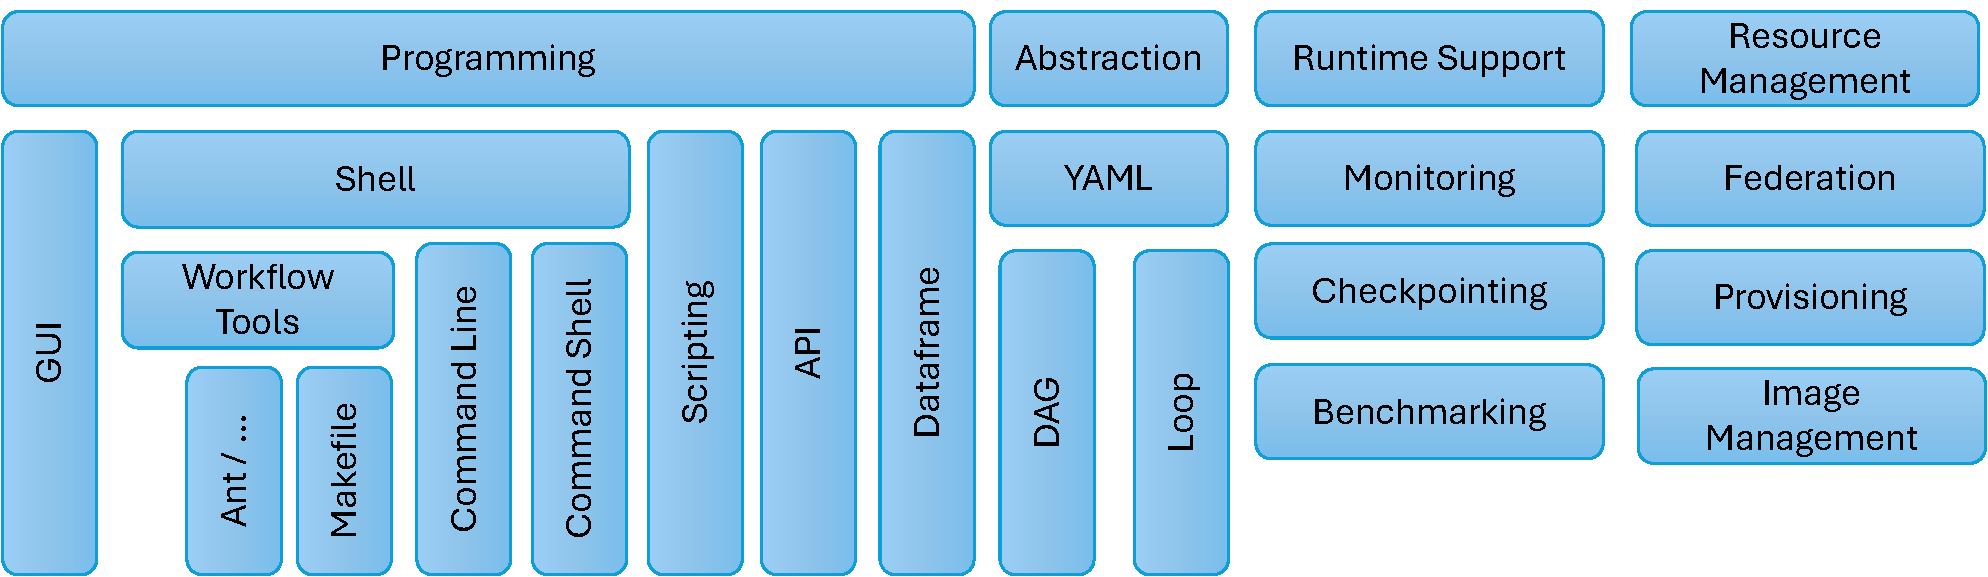
\includegraphics[width=0.70\columnwidth]{images/concepts}
    \caption{Concepts.}
    \label{fig:concepts}
\end{figure}



\begin{figure}[htpb]
  \centering
  \resizebox{0.65\textheight}{!}{%
\begin{forest}
skan tree
   [Supporting Workflow Concepts
        [Abstraction \citep{cloudmesh-ee}
          [YAML
            [DAG]
            [Array
              [Loop]
            ]
          ]
          [Loop]
          [DAG]
        ]
        [Programming
           [GUI]
           [Shell
             [Command line]
             [Command Shell]
             [Tools
                [Makefile]
                [Ant \citep{las-04-gridant}]
                [ ... ]
             ]
           ]
           [Scripting]
           [API \citep{las-02-javacog,las-17-cloudmesh}
             [Python
             [Loop]
             [DAG]
             [Array]
             [AI External Workflow Coordination Frameworks]
             ]
           ]
           [Dataframe \citep{cylon,cylon-radical}]
        ]
        [Runtime Support
           [Monitoring \citep{cloudmesh-ee}]
           [Instrumentation \citep{cloudmesh-stopwatch,cloudmesh-gpu}]
           [Checkpointing \citep{??earthquake}]
           [Benchmarking \citep{cloudmesh-ee}]
           [Reproducability \citep{cloudmesh-ee}]
        ]
        [Resource Management
          [Remote Access \citep{cloudmesh-vpn}]
          [Federation \cite{las-08-federated-cloud,las-12-fedcloud-proc}]
          [Provisioning \citep{las-19-harc-comet,las-17-comet}]
          [Image Management \citep{las-12-imagemanagement}]
          [Scheduling \citep{las-01-greed}]
        ]
   ]
]
\end{forest}
}
   \caption{Scheduling challenges applied to all levels} 
  \label{F:graph-challenges}
\end{figure}



\section{HPC Benchmark  Experiment Workflows}

install software
reserve machine to exclusive use
prepare batch jobs for the run
evaluate and validate the performance
compare results
submit results




%%%%%%%%%%%%%%%%%%%%%%%%%%%%%%%%%%%%%%%%%%%%%%%%%%%%%%%%%%%%%%%%%%%%%%%%%%%%%%%
\subsection{Benchmark Carpentry for Experiment Execution}
%%%%%%%%%%%%%%%%%%%%%%%%%%%%%%%%%%%%%%%%%%%%%%%%%%%%%%%%%%%%%%%%%%%%%%%%%%%%%%%

\textbf{\textit{FAIR}}
When designing benchmarks, it is important to think of the results as experiment data, rather than just an answer to a performance question. Organizing data for later reuse also allows for later application of machine learning to uncover additional insights that can lead to further optimization, e.g., subtle performance gains related to specific software and hardware device combinations. The FAIR Principles provide a framework for aligning research outputs. FAIR is an acronym with 15 underlying principles that relate to Findability, Accessibility, Interoperability, and Reusability (FAIR)\citep{wilkinson2016fair}. More specifically, the FAIR Principles call for use of well-described, standardized metadata, clear licensing and usage information, open or freely available protocols and methods for access, and use of globally unique identifiers. The actual implementation of the FAIR Principles varies by domain, data architecture, and resources available to sustain data management practices and infrastructure \citep{jacobsen2020fair}.

In the case of this work, several practices were identified that relate to making HPC benchmark results more FAIR\citep{kirkpatrick2024}. These include ensuring controlled vocabularies are used when describing system information. Where these are not available, it is preferable for the software, such as cloudmesh, to extract information from other sources, such as system configuration, libraries, or registry settings, especially over use of free form text. Ideally globally, unique identifiers would be assigned to each benchmark output. Other implementations of FAIR can include writing provenance information about how the benchmark was created into the results file.

result templates


%%%%%%%%%%%%%%%%%%%%%%%%%%%%%%%%%%%%%%%%%%%%%%%%%%%%%%%%%%%%%%%%%%%%%%%%%%%%%%%
\section{Experiment Execution Templates}
%%%%%%%%%%%%%%%%%%%%%%%%%%%%%%%%%%%%%%%%%%%%%%%%%%%%%%%%%%%%%%%%%%%%%%%%%%%%%%%

%%%%%%%%%%%%%%%%%%%%%%%%%%%%%%%%%%%%%%%%%%%%%%%%%%%%%%%%%%%%%%%%%%%%%%%%%%%%%%%
\subsection{Experiment Execution on High Performance Computers}
%%%%%%%%%%%%%%%%%%%%%%%%%%%%%%%%%%%%%%%%%%%%%%%%%%%%%%%%%%%%%%%%%%%%%%%%%%%%%%%
In general, users on HPC platforms operate in a computing environment with
fixed computational resources and storage. This strongly influences the types
of experiments that are executed on these platforms which are generally
characterized by inelastic workloads with pre-defined execution.

In particular, users often operate within fixed size allocations (e.g. users
have N node-hours with a pre-specified end date). Executing experiments on
traditional HPC platforms is characterized by submitting batch jobs to the
workload manager (e.g. SLURM or PBS). Additionally, because the amount of work
is largely static, large amounts of resources are allocated for long blocks of
time (hours, days or weeks). Long-running tasks on login nodes are generally
discouraged although more recent HPC platforms include the concept of `workflow'
nodes that can be used to deploy long-running. This leads to experiment
execution following pipeline-like workflows with each batch job submitting a new
batch job to execute the next stage.

HPC users also tend to assume that data is stored locally and in a persistent
state. This allows experiment execution to use the filesystem as a way to swap
data and/or store the state between submissions of batch jobs. Tape archives are
used for long-term storage, however by its nature the time to retrieve large
amounts of data can be cumbersome.

Comparatively speaking, most applications run on bare-metal, i.e. outside of a
container. The main advantage of containers, providing a portable environment,
is less of an issue on HPC platforms which tend to retain the same hardware over
the lifetime of the machine and whose software libraries are updated relatively
infrequently.

%%%%%%%%%%%%%%%%%%%%%%%%%%%%%%%%%%%%%%%%%%%%%%%%%%%%%%%%%%%%%%%%%%%%%%%%%%%%%%%
\subsection{Experiment Execution on Hyperscaler Resources}
%%%%%%%%%%%%%%%%%%%%%%%%%%%%%%%%%%%%%%%%%%%%%%%%%%%%%%%%%%%%%%%%%%%%%%%%%%%%%%%
The increasing availability of resources in the cloud has led to an increased
interest in deploying traditional HPC workloads on hyperscaled resources. These
platforms have traditionally been optimized for web applications where
elasticity of resources is paramount to adapt to dynamically changing workloads.
With the increasing use of the cloud for machine-learning tasks, hardware that
was typically only available on HPC platforms (e.g. high-bandwidth, low-latency
interconnects) are now commonplace. In contrast to traditional HPC, users
have instant access to an (apparently) unlimited amount of computational
resources and storage. 

The elasticity of resources leads to experiment execution paradigms that are
driven by service-oriented architectures. This includes spawning multiple
workers for each service that are ephemeral, often completing a small unit of
work before ending. Applications are loosely coupled with communication and
requests handled through APIs instead of communicating directly with each other.
In contrast to bare-metal HPC, containers are a fundamental requirement to
create customized environments that can be very quickly deployed and scaled onto
a new set of resources. Jobs are usually measured on the order of minutes or
seconds. 

%%%%%%%%%%%%%%%%%%%%%%%%%%%%%%%%%%%%%%%%%%%%%%%%%%%%%%%%%%%%%%%%%%%%%%%%%%%%%%%
\subsection{Federated Experiment Execution}
%%%%%%%%%%%%%%%%%%%%%%%%%%%%%%%%%%%%%%%%%%%%%%%%%%%%%%%%%%%%%%%%%%%%%%%%%%%%%%%

From Grids back to client-side control

%%%%%%%%%%%%%%%%%%%%%%%%%%%%%%%%%%%%%%%%%%%%%%%%%%%%%%%%%%%%%%%%%%%%%%%%%%%%%%%
\subsection{Experiment Execution on Clouds}
%%%%%%%%%%%%%%%%%%%%%%%%%%%%%%%%%%%%%%%%%%%%%%%%%%%%%%%%%%%%%%%%%%%%%%%%%%%%%%%

The CoGKits for Java and Python were the predecessor to cloudmesh. While those tools focused on Grid computing interfaces for the various Grid toolkits. Cloudmesh provided the opportunity to shift its focus to services offered by cloud computing including Azure, AWS, Google, OpenStack clouds, and Chamelon Cloud via OpenStack. Here cloudmesh focused on the creation of a very simple mechanism to start compute resources uniformly on the various clouds while providing templates that offer similar capabilities across them. As such workflows could be created that allowed switching easily be tween virtual machines. This is achieved by the cloudmesh command line and command shell that prior to any other tool allowed integrating and switching between clouds easily. Thus to start a vm on AWS, then one on Azure one could simply say

\begin{verbatim}
cms set cloud=aws
cms vm start
cms set cloud=azures
cms vm start
cms vm start --cloud=google
\end{verbatim}

cloudmesh was the first tool that promoted a setup of cloud credentials in yaml files that were used to start "templated" virtual machines with default parameters provided by these templates. Only later were similar capabilities integrated in for example,  OpenStack. Thus we can support cloud-based workflows

\begin{itemize}
    \item on one or multiple clouds
    \item cloud agnostic workflows
    \item adding easily new clouds into the workflows by integrating access points
    \item allow the integration of new clouds and their vm access protocols
\end{itemize}

As clouds have recently also integrated containers and server less computing we have prototyped the ability to stand up Kubernetes clusters (in AWS for example). As setting up such clusters is a task that is beyond the capabilities of scientists we prototyped an easy way to set them up including default security and network capabilities. The integration into cloudmesh is conducted through the cloudmesh plugin mechanism that ads dynamically this capability with a simple pip install.

Most recently a shift in scientific computing has taken place that emphasizes the use of GPU compute resources. For this reason AWS has added the ability to bootstrap in the cloud parallel clusters including their control through SLURM. Obviously, this could also be leveraged by a scientist that may not have a super computer at their facility or wants to conduct an HPC workload in the cloud. However the configuration and setup is something most scientists do not want to be bothered with. Their goal is the access to the compute resources. Our cloud cluster plugin to cloudmesh therefor contains the ability to deploy a cloud cluster with or without GPUs, as well as the size of the working node with the help of a single command to which we specify such things as the name of the cluster, how many nodes, and if and which GPUs should be used. Obviously that can all be configured through AWS cloud formation, however, the setup and the configuration parameters are too complex to just support this general workflow case. Hence we have provided a simplified YAML configuration file that can also be specified on the command line  and allows reasonable flexibility. One such flexibility is to define multiple clusters that may be busy working on multiple things. It is to be noted that the setup of such cluster costs a significant time (such as 15 minutes) but this is time in contrast to the expected runtimes conducted on such clusters. It also provides a meaningful estimation on when such clusters may be used. For sure, they should not be used by a single user with only a few seconds compute time.  The experiment executions as part of the scientific discover workflow should be much larger.





%%%%%%%%%%%%%%%%%%%%%%%%%%%%%%%%%%%%%%%%%%%%%%%%%%%%%%%%%%%%%%%%%%%%%%%%%%%%%%%
\section{Experiment Executors}
%%%%%%%%%%%%%%%%%%%%%%%%%%%%%%%%%%%%%%%%%%%%%%%%%%%%%%%%%%%%%%%%%%%%%%%%%%%%%%%

\citep{las-frontiers-edu}

%%%%%%%%%%%%%%%%%%%%%%%%%%%%%%%%%%%%%%%%%%%%%%%%%%%%%%%%%%%%%%%%%%%%%%%%%%%%%%%
\subsection{Experiment Executor (Cloudmesh Plugin)}
%%%%%%%%%%%%%%%%%%%%%%%%%%%%%%%%%%%%%%%%%%%%%%%%%%%%%%%%%%%%%%%%%%%%%%%%%%%%%%%

%%%%%%%%%%%%%%%%%%%%%%%%%%%%%%%%%%%%%%%%%%%%%%%%%%%%%%%%%%%%%%%%%%%%%%%%%%%%%%%
\subsection{SmartSim}
%%%%%%%%%%%%%%%%%%%%%%%%%%%%%%%%%%%%%%%%%%%%%%%%%%%%%%%%%%%%%%%%%%%%%%%%%%%%%%%
SmartSim is a Python-based, open-source library that allows users to describe
and execute hybrid AI/ModSim workflows using an in-memory datastore to exchange
data. It has a sibling library SmartRedis that provides C, C++, Fortran, and 
Python clients for simulation and analysis codes to enable components to
communicate with the datastore.

Users describe a workflow by interacting with top-level objects from the
SmartSim library. The highest level object is the ``Experiment'' which contains
factory methods and imperative functions that execute the wokflow. The user can
specify which workload manager (SGE, SLURM, PBSPro, LSF, or a local executor) during
the instantiation of this object. ``Models'' are the Python objects that
represent user applications, for example simulations or Python scripts. Users
can define configurable parameters to modify the behavior of the application
either by modifying its run arguments or by configuring user-tagged files.
Additionally, users can specify files and directories needed to run the
application. ``Ensembles'' extend this concept by allowing users to generate
multiple ``Models''. Lastly, the ``Orchestrator'' object is the in-memory
datastore that provides a central location for workflow components to share
data. This is currently based on Redis. The Redis database can be sharded across
multiple nodes, each one capable of performing inference. Notably requests from
multiple clients can be batched together, minimizing penalties associated with
moving small amounts of data to/from the GPU.

Methods on the ``Experiment'' object configure, execute, and monitor components
of the workflow. The ``generate'' method crease the run directories and copy-in
or symbolically link in files/directories attached to the ``Model'',
``Ensembles'', and ``Orchestrators''. The ``start'' method submits an
instantiated entity to the workload manager. This is non-blocking by default
allowing for the asynchronous execution or can be specified to be blocking.
For more granular control, the ``poll'' and ``get\_status'' methods can also
be used to query the run state of the component.

Combining these entities and methods allows users to create workflows that
cannot be represented by a DAG. For example, new ``Models'' and ``Ensembles''
can be created, configured, and launched dynamically during the execution of the
worfklow. The ``Orchestrator'' can be used to store state and transfer data
between components and stages of the workflow.

%%%%%%%%%%%%%%%%%%%%%%%%%%%%%%%%%%%%%%%%%%%%%%%%%%%%%%%%%%%%%%%%%%%%%%%%%%%%%%%
\section{Evaluation}
%%%%%%%%%%%%%%%%%%%%%%%%%%%%%%%%%%%%%%%%%%%%%%%%%%%%%%%%%%%%%%%%%%%%%%%%%%%%%%%

\subsection{Experiment Executor Features}


\begin{table}[htbp]
\centering
\resizebox{\columnwidth}{!}{%
\begin{tabular}{|l|l|l|}
\hline
\bf Feature &  \makecell{\bf Cloudmesh \\ \bf Experiment Executor and \\\bf Compute Coordinator} &  \bf SmartSim \\
\hline
\multicolumn{3}{|l|}{\cellcolor{gray!20}\bf\em Scheduler}\\
\hline
Queue & SLURM, LSF, SSH, others possible &  SLURM, PBS, LSF, SGE \\
Batch Submission & \YES & \YES \\
Within Allocation & \YES & \YES \\
DAGs  & \YES  & \YES \\
Inferencing Capabilities & \NO & \YES \\
Ensemble execution & \YES & \YES \\
\hline
\multicolumn{3}{|l|}{\cellcolor{gray!20}\bf\em Interface}\\
\hline
Python API & \YES & \YES \\
Command line & \YES & \NO \\
Command shell & \YES & \NO \\
GUI  & (\YES) & \NO \\
\hline
\multicolumn{3}{|l|}{\cellcolor{gray!20}\bf\em Parameters}\\
\hline
YAML & \YES & \YES  \\
multi-value YAML & \YES & \NO \\
Gridsearch & \YES & \YES \\
Customizable & \YES & \YES \\
\hline
\multicolumn{3}{|l|}{\cellcolor{gray!20}\bf\em Federation}\\
\hline
SSH & \YES & \YES \\
Split VPN support & \YES & \NO \\
Build in parallel multi resource experiments & \YES & \NO \\
Combine results by multiple users & \YES & \NO \\
Combine results from multiple resources & \YES & \NO \\
\hline
\multicolumn{3}{|l|}{\cellcolor{gray!20}\bf\em Expandable}\\
\hline
Plugin Manager & \YES & \NO \\
\hline
\multicolumn{3}{|l|}{\cellcolor{gray!20}\bf\em Distribution}\\
\hline
only pip & \YES & Without Redis \\
pip with compile & N/A & With Redis \\
Container & \YES & \YES \\
Singularity & \YES & \YES \\
Docker & \YES & \YES \\
Licence  & Apache 2.0 & BSD-2-Clause license \\
\hline
\multicolumn{3}{|l|}{\cellcolor{gray!20}\bf\em Other Deployments}\\
\hline
AWS Parallel Cluster & \YES & \NO \\ 
AWS Kubernetes  & in progress & \NO \\
\hline
\end{tabular}
}
\caption{Resizable Table with Rotated Column Headers}
\end{table}

\begin{itemize}

\item {\bf Software License Dependencies.} Cloudmesh initially used MongoDB for managing a cached version of its infrastructure. This however had early issues as the documentation and installation instructions for Windows at the time were insufficient and not well documented. We wrote our own installation. Although this was later on improved by MongoDB in 2018 the license was changed and a service model was pushed for revenue purposes. At this time we completely rewrote cloudmesh to use its own internal YAML database based on Python. This allowed 
a much easier pip only install and simplified the setup of cloudmesh drastically. This was also the main issue brought forward by its users to eliminate MongoDB dependencies. 

Recently SmartSim ran into the same problem as it could not distribute Redis on which it currently depends with a precompiled version including containers. Often Alternatives are not available till such licence changes have been made and introduce considerable inconvenience to the existing dependent projects. Currently an alternative to Redis would be KeyDB  \citep{keydb}. 

As a lesson {\em it should be avoided to rely on non public domain software that provide license restrictions.}

At the same time the software to manage the workflows should be distributed under a well known and established open source licence allowing others to also easily contribute. In case of Cloudmesh we have chosen Apache 2.0 due to our good experience for over a decade within many software projects.
Smartsim is distributed under the BSD-2-Clause license.

\end{itemize}



\subsubsection{Cloudmesh Monitoring}
\label{sec:monitoring}

\begin{quote}

TEXT COPIED FROM PREVIOUS PAPER

To conduct monitoring of time we have provided for years a convenient StopWatch package in Python \citep{cloudmesh-stopwatch}.  It is very easy to use and is focused on runtime execution monitoring of time-consuming portions in a single-threaded Python application. Although MLCommons provides their own time measuring component, called mllog, it is clear from the name that the focus is to create entries in a log file that is not easily readable by a human and may require post-processing to make it usable. In contrast, our library contains not only simple labeled \texttt{start} and \texttt{stop} methods, it also provides a convenient mechanism to print human-readable customizable performance tables. However, it is possible to also generate a result table in other formats such as CSV, JSON, YAML, TXT, and others).  Human readability is especially important during a debugging phase when benchmarks are developed. Moreover, we also have developed a plugin interface to mllog, that allows us to automatically create mllog entries into an additional log file, so the data may be used within MLCommons through specialized analytics programs. A use case is depicted next (we have omitted other advanced features such as function decorators for the StopWatch to keep the example simple).



\begin{lstlisting}[language=Python]
    from cloudmesh.common.StopWatch import StopWatch 
    # ...
    StopWatch.event("start")       # this where the timer starts
    StopWatch.start("earthquake")  # this is when the main benchmark starts
    # ... run the earthquake code
    # ... additional timers could be used here
    with StopWatchBlock("calc"):   # this is how to use a block timer
       run_long_calculation()
    StopWatch.stop("earthquake")   # this is where the main benchmark ends
    StopWatch.benchmark()          # prints the current results
\end{lstlisting}

To also have direct access to MLCommons events, we have recently added the ability to call a StopWatch.event.


In addition to the StopWatch, we have developed a simple command line tool that can be used for example in batch scripts to monitor the GPU performance characteristics such as energy, temperature, and other parameters \citep{cloudmesh-gpu}. The tool can be started in a batch script as follows and is currently supporting NVIDIA GPUs:


\begin{lstlisting}[language=sh]
    cms gpu watch --gpu=0 --delay=0.5 --dense > gpu0.log &
\end{lstlisting}


Monitoring time and system GPU information can provide significant insights into the application's performance characteristics. It is significant for planning a time-effective schedule for parameters while running a subset of planned experiments.



\subsubsection{Workflow Compute Coordinator}
\label{sec:workflow-cc}

% possibly some repetition here

Within HPC environments, scientific tasks can leverage the processing power of a supercomputer so they can run at previously unobtainable high speeds or utilize specialized hardware for acceleration that otherwise is not available to the user. HPC can be used for analytic programs that leverage machine learning applied to large data sets to, for example, predict future values or to model current states. For such high-complexity projects, there are often multiple complex programs that may be running repeatedly in either competition or cooperation, as also in the earthquake forecast application.  This may even include resources in the same or different data centers on which the benchmarks are run. To simplify the execution on such infrastructures, we developed a hybrid multi-cloud analytics service framework that was created to manage heterogeneous and remote workflows, queues, and jobs.  It can be used through a Python API, the command line, and a REST service. It is supported on multiple operating systems like macOS, Linux, and Windows 10 and 11.  The workflow is specified via an easy-to-define YAML file.  Specifically, we have developed a library called Cloudmesh Compute Coordinator (cloudmesh-cc) \citep{las-22-arxiv-workflow-cc} that adds workflow features to control the execution of jobs on remote compute resources, while at the same time leveraging capabilities provided by the local compute environments to directly interface with graphical visualizations better suited for the desktop. The goal is to provide numerous workflows that in cooperation enhance the experience of the analytics tasks. This includes a REST service (see Figure \ref{fig:cc-3}A) and command line tools to interact with it.


% FIG 5
\begin{figure}[htb]


  \ifbool{SUBMISSION}{
    \centering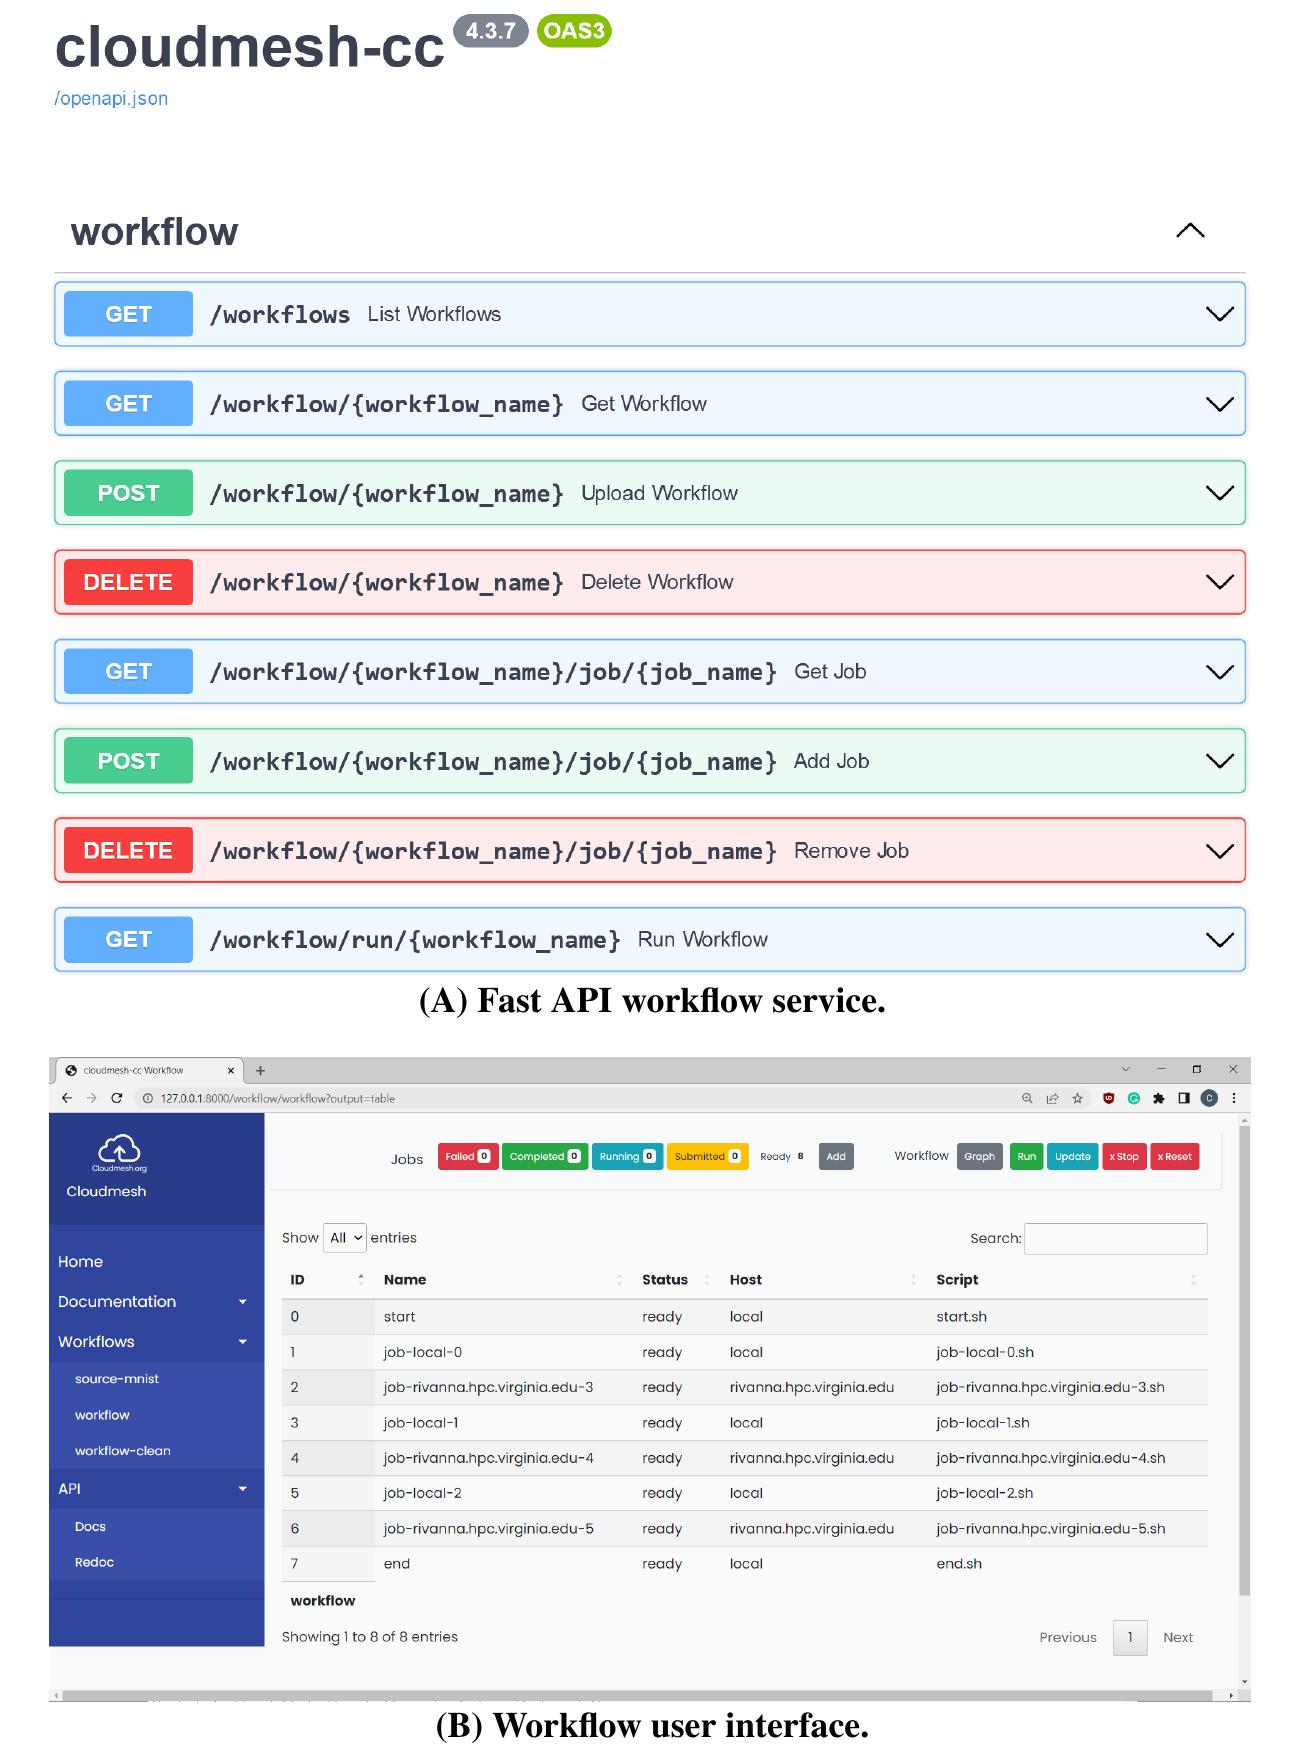
\includegraphics[width=0.8\columnwidth]{images/fig5.jpg}
}{

    \centering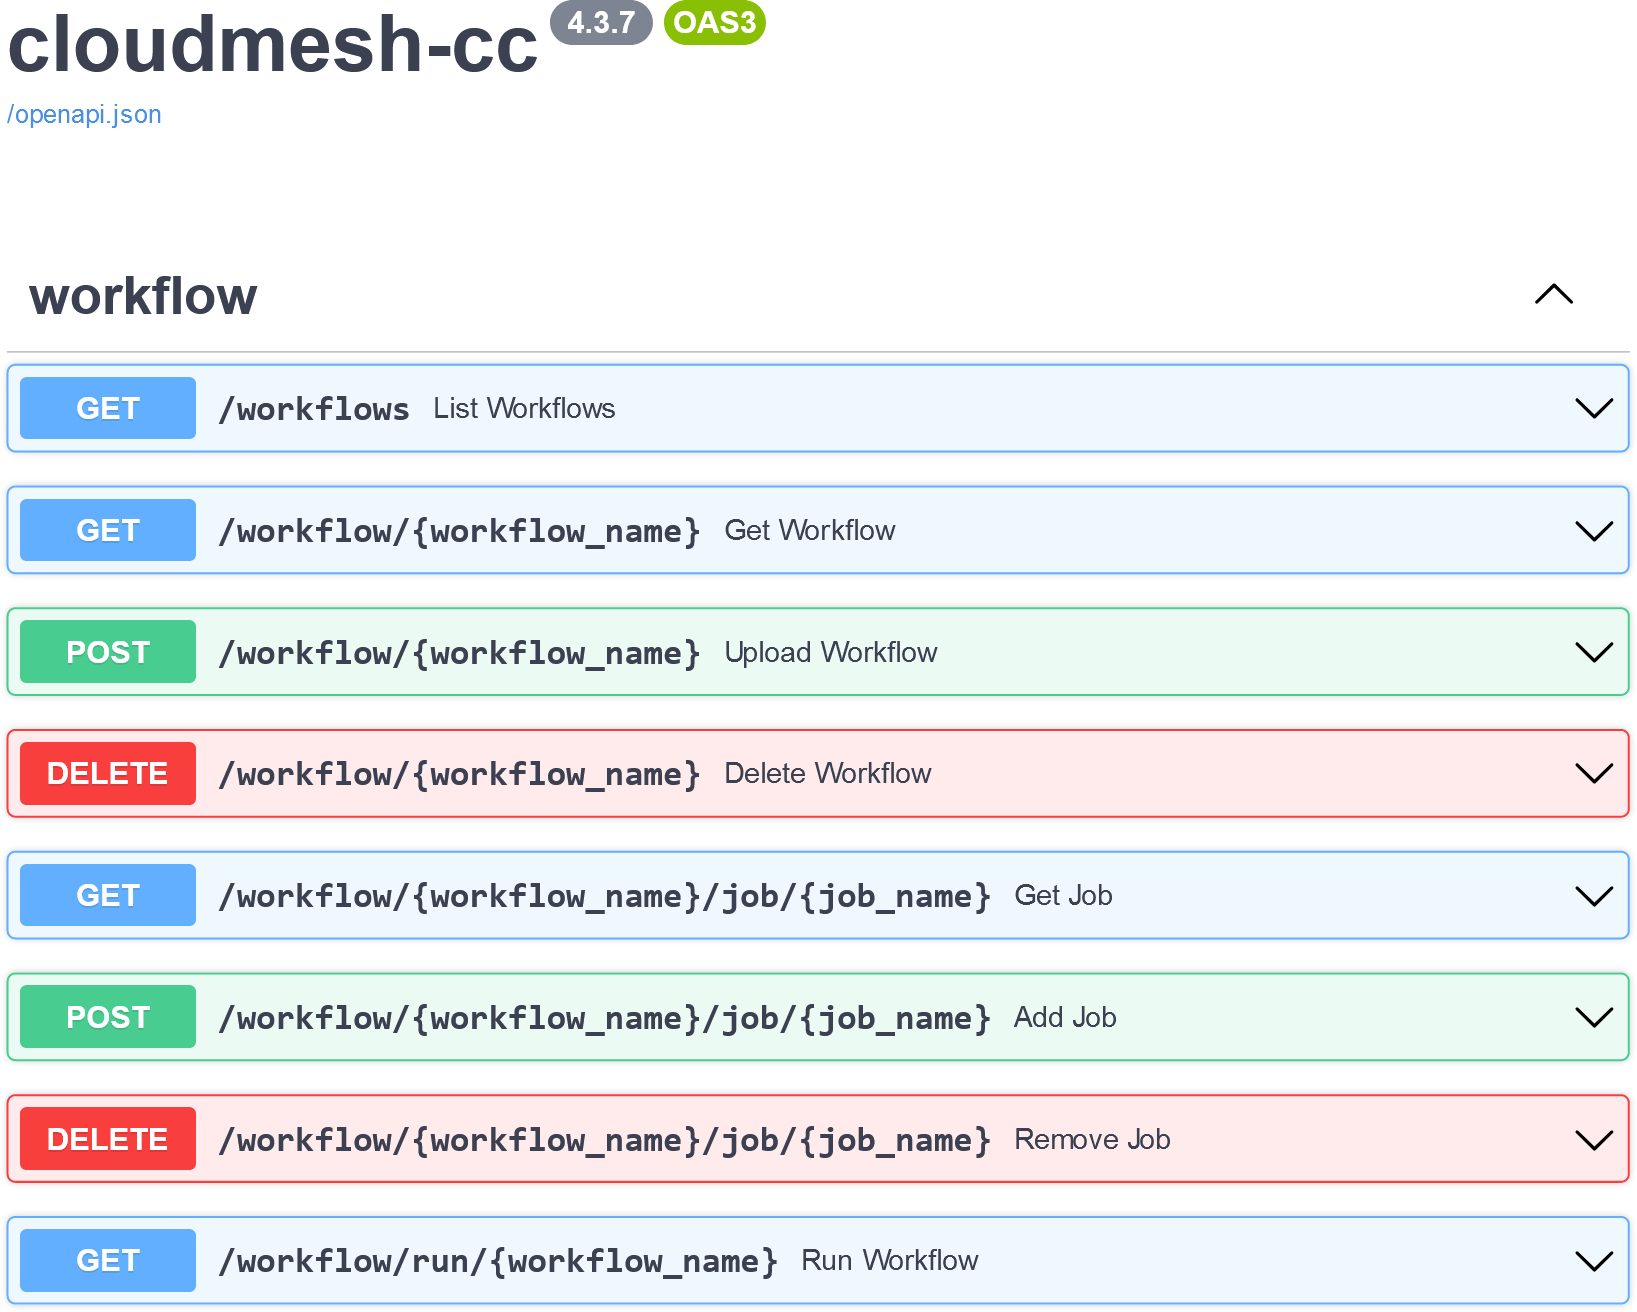
\includegraphics[width=0.8\columnwidth]{images/fastapi-service-highres.jpg}
    
    {\bf (A) Fast API workflow service.}

  \bigskip


    \centering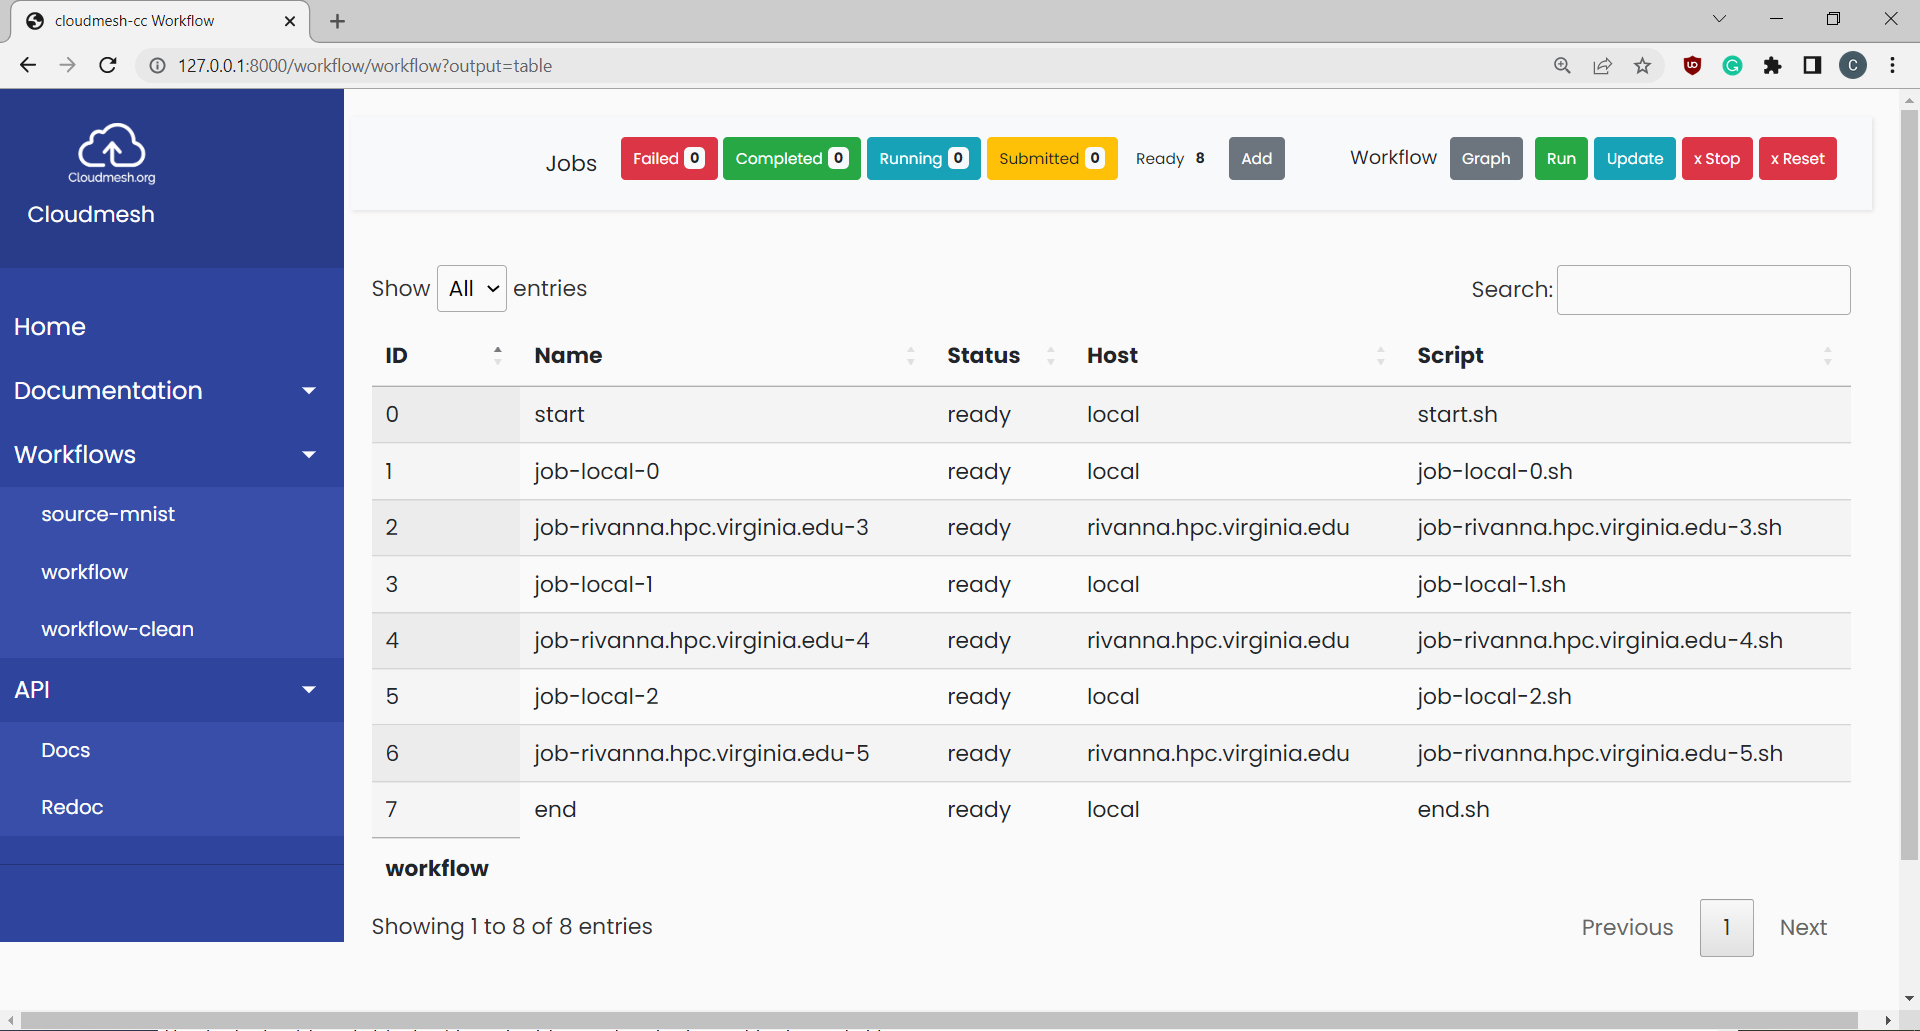
\includegraphics[width=0.8\columnwidth]{images/cc-1.jpg}

    {\bf (B) Workflow user interface.}

}
  

    \caption{Workflow interfaces.}
    \label{fig:cc-3}
\end{figure}


We have tested the framework while running various MNIST application examples, including Multilayer Perceptron, LSTM (Long short-term memory), Auto-Encoder, Convolutional, and Recurrent Neural Networks, Distributed Training, and PyTorch training.  A much larger application using earthquake prediction has also been used.
Recently the framework was applied by students to all applications in the MLCommons Applications working group. Results of using it outside of the earthquake code are available in \cite{las-2023-escience}.

Figure \ref{fig:cc-3}A shows the REST specification and \ref{fig:cc-3}B shows the graphical user interface.

\subsubsection{Parameterized Experiment Workflow Job Generator}
\label{sec:workflow-ee}

In traditional machine learning workflows, hyperparameter tuning and configuration are key elements in assessing and optimizing the performance of models. However, scaling hyperparameters for highly parallel execution with heterogeneous hardware is complex.

Cloudmesh-ee \cite{cloudmesh-ee,las-2023-escience} is a hyperparameter and configuration management toolkit designed to address the generation of batch jobs with a consistent and configurable interface based on hyperparameter values across multiple development toolchains. One of its functions is to create batch jobs based on parameterized job specifications and configuration files.  Cloudmesh-ee is part of the Cloudmesh toolkit, a set of tools and libraries for managing cloud and HPC resources from the command line, REST interfaces, or GUI's.  Cloudmesh-ee can use a variety of queuing systems and submission commands. Currently, we provide interfaces to Slurm, LSF, and ssh. 

The architecture of the cloudmesh-ee framework is depicted in Figure \ref{fig:cc-2}B.

Cloudmesh-ee differentiates itself from other approaches through its ability to generate a cartesian product (permutation) of hyperparameter to form independent {\it experiment} execution profiles, making it trivial to scale an experiment from one execution to thousands of configurations based on the ranges and their unique combinations.  The resulting output provides a generated Slurm or LSF script and a YAML configuration file representing the specific hyperparameters.  By managing many highly configurable jobs with cloudmesh-ee, the focus is placed on what hyperparameters to use for experiments and reduce the possibility of human error when running experiments over a range of hyperparameters.

Cloudmesh-ee takes two configuration files. The first is a YAML file that includes all parameters used by the benchmark including an experiment section that defines the cartesian product. The second is a slurm template. From these files, it will create Slurm scripts via the cloudmesh-ee commandline tool while

\begin{enumerate}
  \item using a unique directory for the experiment
  \item taking a parameter set from the cartesian product of the experiment parameters
  \item creating from a batch job template an instantiation of the template while replacing all variables from the configuration file    and replacing the specific experiment parameters
  \item creating an instantiation of the configuration file while replacing all experiment parameters with the one for the current experiment.
\end{enumerate}

This is executed for all permutations of the experiment parameters.

An example of a configuration file \verb|config.yaml| where we iterate over epochs, gpus, and repeat it 5 times is shown next:

\begin{lstlisting}
    application:
        name: earthquake

    data: /scratch/{os.USER}/{application.name}
       
    experiment:
        epoch: "1,30,60"
        gpu: "a100,v100"
        repeat: "1,2,3,4,5"
\end{lstlisting}

An example of a batch script in the cloudmesh template markup  is:

\begin{lstlisting}[language=sh]
    #!/bin/bash

    #SBATCH --job-name={experiment.repeat}-{application.earthquake}
    #SBATCH --nodes=1
    #SBATCH --gres=gpu:{experiment.gpu}:1
    #SBATCH --time=02:00:00
    #SBATCH --mem=64G
    #SBATCH -o {experiment.gpu}-{application.earthquake}/{experiment.repeat}-%j.out
    #SBATCH -o {experiment.gpu}-{application.earthquake}/{experiment.repeat}-%j.err
    #SBATCH --partition=bii-gpu
    #SBATCH --account=bii_dsc_community

    export USER_SCRATCH=/scratch/$USER
    cd USER_SCRATCH
    mkdir -p $USER_SCRATCH/{experiment.gpu}-{application.earthquake}/%j.out
    (*\textcolor{blue}{nvidia-smi}*)

    cms gpu watch --gpu=0 --delay=0.5 --dense > outputs/gpu0.log &

    python earthquake.py --config config.yaml

    seff $SLURM_JOB_D
\end{lstlisting}
%$

The variables can easily be referred to with a dot notation in the templates.  Variables in the YAML file can also be replaced so it is possible to use abbreviations easily and in a consistent fashion in the YAML file as well as in the batch script.

The configuration files and cloudmesh-ee can be configured with parameters so that the files and directories are placed in the right location and repeatable experiments are created not only on the original machine but the template can also be easily adapted onto other machines. An example of a variable replacement specification in the YAML file is given for the \verb|data| value where not only the operating system variable \verb|os.USER| is replaced, but also the variable \verb|{application.name}|. Obviously, this is a significant functionality enhancement to a typical YAML file.  Multiple values are only possible under the experiment tag, where a variable with multiple values is assigned a string of comma-separated values.

One can choose a number of important parameters as part of the permutation strategy to create different experiments. Common variables are names of graphics cards (if available), memory, file systems used, versions of Python, versions of TensorFlow, epochs, learning rate, and many other important parameters that can influence the benchmark.  The reason why we only allow the parameters with variation under \verb|experiment| is to ensure that there is no confusion with other parameters that may not be modified and instead only represent a single value. However, variables under experiment are also allowed to have just a single value.  Another interesting case is the introduction of a repeat parameter, allowing the program to be executed multiple times in order to for example support patterns of competition or collaboration while selecting the best values, or creating averages.


The final output of cloudmesh-ee is a shell script that contains all jobs that are to be executed with the defined permutations over the parameters. One nice side effect of this is that the jobs in the file can be run in parallel and have the queuing system take over the scheduling of the job following the system-defined queuing policies. However, it may also be possible to create a {\it collaborative group} submission, using our earlier introduced collaborative pattern, where multiple users submit a portion of the jobs so that policies restricting the number of jobs per user can be avoided. Furthermore, if access to multiple HPC machines is available the jobs could be split among the different machines. However, in that case, time measurements may not be a useful parameter to benchmark. However, as in the science group, we are concerned about accuracy the combination of a system comprised of multiple resources is meaningful.

Our progress with the earthquake benchmark would not have been possible if we did not have cloudmesh-ee to coordinate the many experiments in a consistent fashion. One important aspect is that the management of thousands of jobs that we ran was simplified and the jobs could be created easily while fostering reproducibility. The resulting jobs were run over a time period of a month, while each job took many hours to complete.

We have practical experience from multiple teams where coders spent multiple months developing programs and strategies to coordinate their experiment executions; to circumvent this expenditure, the cloudmesh experiment executor generated such permutations within one day on a variety of systems.

\end{quote}

%%%%%%%%%%%%%%%%%%%%%%%%%%%%%%%%%%%%%%%%%%%%%%%%%%%%%%%%%%%%%%%%%%%%%%%%%%%%%%%
\subsection{Applications}
%%%%%%%%%%%%%%%%%%%%%%%%%%%%%%%%%%%%%%%%%%%%%%%%%%%%%%%%%%%%%%%%%%%%%%%%%%%%%%%


%%%%%%%%%%%%%%%%%%%%%%%%%%%%%%%%%%%%%%%%%%%%%%%%%%%%%%%%%%%%%%%%%%%%%%%%%%%%%%%
\subsubsection{OSMI}
%%%%%%%%%%%%%%%%%%%%%%%%%%%%%%%%%%%%%%%%%%%%%%%%%%%%%%%%%%%%%%%%%%%%%%%%%%%%%%%

Most AI workflows on HPC can be categorized in six different execution motifs: Steering, Multistage Pipeline, Inverse Design, Digital Replica, Distributed Models, and Adaptive Training \cite{brewer2024ai}. One component that shows up across multiple motifs is machine-learned surrogate models. Such models typically are used in hybrid ModSim / AI workflows, where traditional simulations are used for a large part of the workflow, and then particular aspects of the simulation, such as a turbulence or radiation model, are replaced by digital surrogates, e.g., \cite{partee2022using, martinez2022roam, bhushan2023assessment}. Because of the challenges of integrating the simulations with the AI model in a highly scalable manner, developing a benchmark was necessary to assess the performance of various configurations. Initial developments of a surrogate model benchmark, called ``OsmiBench'', were studied by Brewer et al. \cite{brewer2021production}. The studies showed that using a separate load balancer on each compute node, which round-robins the inference requests across multiple GPUs on the node, and also using the maximum batch size that the GPU memory allows yields optimal inference performance. This study was followed by a secondary investigation by Boyer et al. \cite{boyer2022scalable}, which investigated performance implications of the full coupling between the surrogate inference and the simulation code, and showed that using a concurrency level of two batch inference requests was optimal. 

The Open Surrogate Model Inference (OSMI) benchmark was developed as an open-source community benchmark founded upon these principles. The architecture of OSMI is shown in Fig. \ref{fig:osmi}. The benchmark supports either TensorFlow or SmartSim/PyTorch based frameworks as shown in Table \ref{tab:osmi}. Inference requests are initiated from within the simulation using a client API call (e.g., SmartRedis or gRPC API), the requests are then sent to a load balancer (e.g., HAProxy), which distributes the requests in a round-robin fashion to multiple inference servers, each bound to a single GPU. Benchmark timings are able to be measured at multiple places in the architecture, but the primary measurement of interest is how long it takes from the time an inference request is initiated from the simulation, until the response is returned back to it. As opposed to chip-level benchmarks such as MLPerf \cite{reddi2020mlperf}, OSMI is able the measure system-level performance, which includes the performance of the CPU, GPU, network, and interconnect (IC), giving a holistic performance representation of the system. This same approach was used to benchmark a wide range of HPC systems, revealing significant performance differences between seemingly similar machines, often due to factors such as different interconnect performance \cite{brewer2020inference}.

\begin{figure}[t]
    \centering
    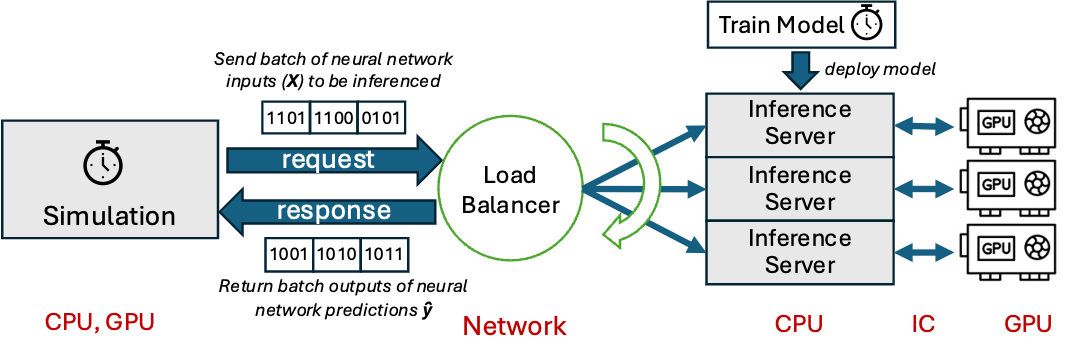
\includegraphics[width=\linewidth]{images/osmi_arch.png}
    \caption{Architecture of OSMI benchmark.}
    \label{fig:osmi}
\end{figure}

\begin{table}[t]
\centering
\renewcommand{\arraystretch}{1.5}
\begin{tabular}{llll}
\hline
\textbf{AI framework} & \textbf{Inference server} & \textbf{Client API} & \textbf{Protocol} \\ \hline
TensorFlow & TF Serving  & TF Serving API  & gRPC  \\
PyTorch    & RedisAI     & SmartRedis      & RESP  \\ \hline
\end{tabular}
\caption{OSMI-supported AI frameworks.}
\label{tab:osmi}
\end{table}

%%%%%%%%%%%%%%%%%%%%%%%%%%%%%%%%%%%%%%%%%%%%%%%%%%%%%%%%%%%%%%%%%%%%%%%%%%%%%%%
\subsubsection{Cyclic Execution }
%%%%%%%%%%%%%%%%%%%%%%%%%%%%%%%%%%%%%%%%%%%%%%%%%%%%%%%%%%%%%%%%%%%%%%%%%%%%%%%

Workflow execution has typically focused on workflows that can be represented by
a pipeline or more generally a directed acyclic graph (cycles with predefined
loop limits can be unrolled). Many solutions exist to execute and monitor these
types of workflows (e.g. Parsl or Maestro). In both these cases, the execution
is deterministic.

Other types of workflows, becoming more popular in scientific applications,
involve branches or criteria based loops, thus violating the fundamental
assumptions of a DAG. One common application is automatic parameter estimation.
For example in \citep{Maric2024OpenFOAM}, a Bayesian optimizer is applied to
an OpenFOAM computational fluid dynamics case. The optimizer at every iteration
generates candidate parameter sets which are then used to launch new cases. The
output form those cases are then ingested by the optimizer for the next
iteration. As is typical of optimization problems, this cycle ends when either
the loss function converges, stalls, or reaches a certain number of
optimizations.

Reinforcement learning is another type of workflow which involves non-cyclic
and potentially branching workflow execution. In \citep{Font2024}, an ML
model is used to control the behavior of a turbulent flow surrounding a rising
bubble. The ML model is able to modify the flow by controlling actuators.
The RL model deploys multiple agents in the various environments to explore
and refine the optimal actions. Similarly, \citep{Kurz2022} train a surrogate
model of turbulence using an RL framework. The agent predicts an eddy viscosity
where the RL model is incentivized to match the energy spectra in a
turbulence-resolving model. As in \citep{Font24}, the scientific simulation is
used as an environment to evaluate the agents' strategies. In both these cases,
the need to continue to iterate and test requires dynamic configuration and
execution where the number of cycles is not known a priori.



%%%%%%%%%%%%%%%%%%%%%%%%%%%%%%%%%%%%%%%%%%%%%%%%%%%%%%%%%%%%%%%%%%%%%%%%%%%%%%
\subsection{Community Experience}
%%%%%%%%%%%%%%%%%%%%%%%%%%%%%%%%%%%%%%%%%%%%%%%%%%%%%%%%%%%%%%%%%%%%%%%%%%%%%%%

%%%%%%%%%%%%%%%%%%%%%%%%%%%%%%%%%%%%%%%%%%%%%%%%%%%%%%%%%%%%%%%%%%%%%%%%%%%%%%%
\section{Related Activities}
%%%%%%%%%%%%%%%%%%%%%%%%%%%%%%%%%%%%%%%%%%%%%%%%%%%%%%%%%%%%%%%%%%%%%%%%%%%%%%%


%%%%%%%%%%%%%%%%%%%%%%%%%%%%%%%%%%%%%%%%%%%%%%%%%%%%%%%%%%%%%%%%%%%%%%%%%%%%%%%
\section{Future Work}
%%%%%%%%%%%%%%%%%%%%%%%%%%%%%%%%%%%%%%%%%%%%%%%%%%%%%%%%%%%%%%%%%%%%%%%%%%%%%%%


%%%%%%%%%%%%%%%%%%%%%%%%%%%%%%%%%%%%%%%%%%%%%%%%%%%%%%%%%%%%%%%%%%%%%%%%%%%%%%%
\section{Conclusion}
%%%%%%%%%%%%%%%%%%%%%%%%%%%%%%%%%%%%%%%%%%%%%%%%%%%%%%%%%%%%%%%%%%%%%%%%%%%%%%%



%%%%%%%%%%%%%%%%%%%%%%%%%%%%%%%%%%%%%%%%%%%%%%%%%%%%%%%%%%%%%%%%%%%%%%%%%%%%%%%
\clearpage

\section{Nomenclature}

\subsection{Resource Identification Initiative}

{\bf Organization:} \verb|RRID:SCR_011743|

\section*{Conflict of Interest Statement}

The authors declare that the research was conducted in the absence of any commercial or financial relationships that could be construed as a potential conflict of interest.

\section*{Author Contributions}

{\em GvL} is the author of the Experiment Executor and many other components that are distributed at bag of plugins to cloudmesh.  He has modified modifications to how the OSMI benchmark operates while leveraging some of the elementary features contained in the cloudmesh experiment management. He has decades worth of HPC dating back to 1984. 

{\em GCF} is the author of the earthquake code and facilitates the interactions with the MLCommons Science Working group as a group leader of that effort. 


{\em WB} is the author of the OSMI code and benchmark. His experience from using DOE machines is integrated into this paper. {AS} is the author of SmartSim and his experience from supporting the many customers in HPE is integrated into this paper.

\section*{Funding}

Work was in part funded by the NSF CyberTraining: CIC: CyberTraining for Students and Technologies from Generation Z with the award numbers 1829704 and 2200409 and NIST 60NANB21D151T.  The work was also funded by the Department of Energy under the grant Award No. DE-SC0023452. The work was conducted at the Biocomplexity Institute and Initiative at the University of Virginia.

\section*{Acknowledgments}

We like to thank Jaques P. Fleisher for his contribution to the cloudmesh-vpn plugin for integrating split VPN as well as his independent testing of the workflow code for multiple scientific applications such as earthquake and cloudmask.

This research was sponsored in part by and used resources of the Oak Ridge Leadership Computing Facility (OLCF), which is a DOE Office of Science User Facility at the Oak Ridge National Laboratory (ORNL) supported by the U.S. Department of Energy under Contract No. DE-AC05-00OR22725.

\section*{Data Availability Statement}

The code is all in the public domain and available on GitHub at the following locations

\begin{itemize}

\item {\bf cloudmesh-cc} -- Is a code to control workflows to be executed on
  remote computing
  resources. \url{https://github.com/cloudmesh/cloudmesh-cc}

\item {\bf cloudmesh-ee} -- Is a code to generate batch scripts for
  hyperparameter studies high-performance computers so they can be
  executed on different supercomputers by multiple
  accounts. \url{https://github.com/cloudmesh/cloudmesh-ee}


\item {\bf cloudmesh-vpn} -- Is a plugin that allows to use a VPN client as part of the client focused workflow supported by the cloudmesh command and shell. Recently we added support for split VPN allowing the access to multiple resources controlled by multiple VPNs.
\url{https://github.com/cloudmesh/cloudmesh-vpn}

\item {\bf cloudmesh} -- Cloudmesh is a large collection of repositories for
  accessing cloud and HPC
  resources. \url{https://github.com/orgs/cloudmesh/repositories}

\item {\bf OSMI} -- Is a surrogate-model inference benchmark. \url{https://github.com/laszewsk/osmi-bench-new}

%\item {\bf MLCommons earthquake production code} -- The MLCommons Science
%  Working group is described at
%  \url{https://mlcommons.org/en/groups/research-science/}. This page
%  contains the links to the production-level earthquake code.

%\item {\bf MLCommons earthquake development code} -- The development version of
%  the code is available in this repository. It also contains many of
%  the analysis scripts that are not part of the production code
%  hosted by MLCommons \url{https://github.com/laszewsk/mlcommons}.

\end{itemize}

%\section{Workflow Use case for Parallel Cluster in Amazon}
%Harshad writes after README.md completed
AWS Parallel Computing service (PCS) simplifies the infrastructure deployment of High Performance Computing (HPC) clusters on Amazon Web service cloud infrastructure. \citep{awspcs} It creates an abstraction layer for the end user such as scientists who intend to run their simulations and analyze results of experiments. So they can focus on the outcomes of the experiments rather than spending time in building infrastructure required to run their experiments. The cloudmesh create plugin provides necessary automation that enables users to deploy clusters within minutes. Using cloudmesh create a fully functional PCS cluster can be  built in about 6 minutes. 

The cloudmesh create plugin not only automates the cluster creation process, it goes much beyond that. It creates a head node that, a worker node-group with a minimum capacity of 0 and a  queue. The worker node minimum capacity of 0 is intentional in order to keep cloud costs in control. Users can login to head node to interact with the cluster, submit Simple Linux Utility for Resource Management (SLURM) jobs. This provides users with a seamless experience that they are used to work with on-premise HPC clusters. The nodes of the HPC can utilize a variety of compute options, starting from low cost options for basic compute performance to the highest level of performance provided by Graphical Processing Unit (GPU) based instances.

Shared Storage options

PCS can be used for a variety of use cases such as   

PCS pricing involves two components primarily, first the per hour charge for the PCS managed service itself which includes the controller fee as well as node management fee, and secondly per hour charge for the compute instances. Controller fee depends on the size of the cluster in terms of number of nodes. There are 3 size options for controller available, small medium and large and the price ranges from \$0\.60 to \$6\.7 per hour. Node management fee is either \$0.08 per hour for standard or \$0.66 per hour for advanced. \citep{HPCpricing} Charge for the second component depend on the type of instances being utilized, for example a t2.micro instance with 1 vCPU and 1 GB RAM is eligible for a free tier and does not incur any cost while higher compute instances such as G6 type that come with NVIDIA L4 Tensor Core GPU's would cost much higher, as high as \$13 per hour. \citep{ec2ondemand} In cases where users have flexibility to schedule jobs, they can take advantage of spot instances. PCS and the automation offered by cloudmesh create allow users to choose between on demand and spot instances, spot instance can provide savings in the range of 60-70\%. \citep{spotSavings:online}



%\section{Workflow Use case for EKS Cluster in Amazon}
%Harshad writes after README.md completed



% \bibliographystyle{Frontiers-Harvard}

\bibliographystyle{Frontiers-Vancouver} % Many Frontiers journals
% use the numbered referencing system, to find the style and resources
% for the journal you are submitting to:
% https://zendesk.frontiersin.org/hc/en-us/articles/360017860337-Frontiers-Reference-Styles-by-Journal

\bibliography{%
vonLaszewski-frontiers-citations,%
vonLaszewski-jabref-2021-withnoteurls,%
vonLaszewski-harshadpitkar}





\end{document}
